\documentclass[a4paper, 14pt]{extarticle}

% Поля
%--------------------------------------
\usepackage{geometry}
\geometry{a4paper,tmargin=2cm,bmargin=2cm,lmargin=3cm,rmargin=1cm}
%--------------------------------------


%Russian-specific packages
%--------------------------------------
\usepackage[T2A]{fontenc}
\usepackage[utf8]{inputenc} 
\usepackage[english, main=russian]{babel}
%--------------------------------------

\usepackage{textcomp}

% Красная строка
%--------------------------------------
\usepackage{indentfirst}               
%--------------------------------------             


%Graphics
%--------------------------------------
\usepackage{graphicx}
\graphicspath{ {./images/} }
\usepackage{wrapfig}
%--------------------------------------

% Полуторный интервал
%--------------------------------------
\linespread{1.3}                    
%--------------------------------------

%Выравнивание и переносы
%--------------------------------------
% Избавляемся от переполнений
\sloppy
% Запрещаем разрыв страницы после первой строки абзаца
\clubpenalty=10000
% Запрещаем разрыв страницы после последней строки абзаца
\widowpenalty=10000
%--------------------------------------

%Списки
\usepackage{enumitem}

%Подписи
\usepackage{caption} 

%Гиперссылки
\usepackage{hyperref}

\hypersetup {
	unicode=true
}

%Рисунки
%--------------------------------------
\DeclareCaptionLabelSeparator*{emdash}{~--- }
\captionsetup[figure]{labelsep=emdash,font=onehalfspacing,position=bottom}
%--------------------------------------

\usepackage{tempora}

%Листинги
%--------------------------------------
\usepackage{listings}
\lstset{
  basicstyle=\ttfamily\footnotesize, 
  %basicstyle=\footnotesize\AnkaCoder,        % the size of the fonts that are used for the code
  breakatwhitespace=false,         % sets if automatic breaks shoulbd only happen at whitespace
  breaklines=true,                 % sets automatic line breaking
  captionpos=t,                    % sets the caption-position to bottom
  inputencoding=utf8,
  frame=single,                    % adds a frame around the code
  keepspaces=true,                 % keeps spaces in text, useful for keeping indentation of code (possibly needs columns=flexible)
  keywordstyle=\bf,       % keyword style
  numbers=left,                    % where to put the line-numbers; possible values are (none, left, right)
  numbersep=5pt,                   % how far the line-numbers are from the code
  xleftmargin=25pt,
  xrightmargin=25pt,
  showspaces=false,                % show spaces everywhere adding particular underscores; it overrides 'showstringspaces'
  showstringspaces=false,          % underline spaces within strings only
  showtabs=false,                  % show tabs within strings adding particular underscores
  stepnumber=1,                    % the step between two line-numbers. If it's 1, each line will be numbered
  tabsize=2,                       % sets default tabsize to 8 spaces
  title=\lstname                   % show the filename of files included with \lstinputlisting; also try caption instead of title
}
%--------------------------------------

%%% Математические пакеты %%%
%--------------------------------------
\usepackage{amsthm,amsfonts,amsmath,amssymb,amscd}  % Математические дополнения от AMS
\usepackage{mathtools}                              % Добавляет окружение multlined
\usepackage[perpage]{footmisc}
%--------------------------------------

%--------------------------------------
%			НАЧАЛО ДОКУМЕНТА
%--------------------------------------

\begin{document}

%--------------------------------------
%			ТИТУЛЬНЫЙ ЛИСТ
%--------------------------------------
\begin{titlepage}
\thispagestyle{empty}
\newpage


%Шапка титульного листа
%--------------------------------------
\vspace*{-60pt}
\hspace{-65pt}
\begin{minipage}{0.3\textwidth}
\hspace*{-20pt}\centering

\includegraphics[width=\textwidth]{emblem}
\end{minipage}
\begin{minipage}{0.67\textwidth}\small \textbf{
\vspace*{-0.7ex}
\hspace*{-6pt}\centerline{Министерство науки и высшего образования Российской Федерации}
\vspace*{-0.7ex}
\centerline{Федеральное государственное бюджетное образовательное учреждение }
\vspace*{-0.7ex}
\centerline{высшего образования}
\vspace*{-0.7ex}
\centerline{<<Московский государственный технический университет}
\vspace*{-0.7ex}
\centerline{имени Н.Э. Баумана}
\vspace*{-0.7ex}
\centerline{(национальный исследовательский университет)>>}
\vspace*{-0.7ex}
\centerline{(МГТУ им. Н.Э. Баумана)}}
\end{minipage}
%--------------------------------------

%Полосы
%--------------------------------------
\vspace{-25pt}
\hspace{-35pt}\rule{\textwidth}{2.3pt}

\vspace*{-20.3pt}
\hspace{-35pt}\rule{\textwidth}{0.4pt}
%--------------------------------------

\vspace{1.5ex}
\hspace{-35pt} \noindent \small ФАКУЛЬТЕТ\hspace{80pt} <<Информатика и системы управления>>

\vspace*{-16pt}
\hspace{47pt}\rule{0.83\textwidth}{0.4pt}

\vspace{0.5ex}
\hspace{-35pt} \noindent \small КАФЕДРА\hspace{50pt} <<Теоретическая информатика и компьютерные технологии>>

\vspace*{-16pt}
\hspace{30pt}\rule{0.866\textwidth}{0.4pt}
  
\vspace{11em}

\begin{center}
\Large {\bf Лабораторная работа № 8} \\ 
\large {\bf по курсу <<Языки и методы программирования>>} \\
\large <<Разработка шаблона класса>> \\
\Large Вариант 7
\end{center}\normalsize

\vspace{8em}


\begin{flushright}
  {Студент группы ИУ9-21Б Шиятов Н. \hspace*{15pt}\\ 
  \vspace{2ex}
  Преподаватель Посевин Д. П.\hspace*{15pt}}
\end{flushright}

\bigskip

\vfill
 

\begin{center}
\textsl{Москва 2023}
\end{center}
\end{titlepage}
%--------------------------------------
%		КОНЕЦ ТИТУЛЬНОГО ЛИСТА
%--------------------------------------

\renewcommand{\ttdefault}{pcr}

\setlength{\tabcolsep}{3pt}
\newpage
\setcounter{page}{2}

\section{Задание}\label{Sect::task}

Необходимо составить шаблон класса,
перегрузив указанные операции. Проверку работоспособности класса
требуется организовать в функции main, размещённой в файле «main.cpp».

PtrQueue<T> – очередь указателей на структуры
типа T, реализованная через кольцевой буфер.
Операции, которые должны быть перегружены
для PtrQueue<T>:
\begin{enumerate}
    \item «$\ll$» -- добавление указателя на в очередь (enqueue);
    \item «$\text{!}$» -- вытаскивание указателя из очереди (dequeue);
    \item empty -- проверка на пустоту очереди;
    \item унарный «$\ast$ » -- возвращает значение, адрес которого лежит в начале очереди (туда указывает head);
    \item «$-\textgreater$» -- осуществляет доступ к полям структуры, адрес которой лежит в начале очереди.
\end{enumerate}

\section{Результаты}\label{Sect::res}

Исходный код программы представлен в листингах~\ref{lst:queue}--~\ref{lst:main}.

Результат запуска представлен на рисунке~\ref{fig:output}.

\begin{figure}[!htb]
\begin{lstlisting}[language=Java,caption={Класс PtrQueue},label={lst:queue}]
template<typename T>
class PtrQueue {
private:
    T **data;
    int head, tail, max_size;
public:
    PtrQueue(int size) {
        data = new T*[size];
        max_size = size;
        head = 0;
        tail = 0;
    }
    
    bool empty() {
        return head == tail;
    }

    friend PtrQueue<T>& operator<<(PtrQueue<T> &queue, T *ptr) {
        queue.data[queue.tail] = ptr;
        queue.tail = (queue.tail + 1) % queue.max_size;
        return queue;
    }

    friend T* operator!(PtrQueue<T> &queue) {
        T *ptr = queue.data[queue.head];
        queue.head = (queue.head + 1) % queue.max_size;
        return ptr;
    }

    T* operator*() {
        if (empty()) {
            return 0;
        }
        return data[head];
    }

    T* operator->() {
        if (empty()) {
            return 0;
        }
        return data[head];
    }
};
\end{lstlisting}
\end{figure}

\begin{figure}[!htb]
\begin{lstlisting}[language={},caption={Проверка работоспособности},label={lst:main}]
#include "PtrQueue.cpp"

#include <iostream>
using namespace std;

struct Point {
    int x;
    int y;
};

int main() {
    PtrQueue<Point> queue1(3);
    PtrQueue<Point> queue2(3);
    
    Point point1 = {1, 2};
    Point point2 = {7, 8};
    
    Point point3 = {5, 6};
    Point point4 = {9, 0};
    
    queue1 << &point1;
    queue1 << &point2;
    
    queue2 << &point3;
    queue2 << &point4;
    
    
    Point *p1 = *queue1;
    Point *p2 = !queue1;
    Point *p3 = *queue2;
    Point *p4 = !queue1;
    
    
    cout << "p1->x = " << p1->x << endl;
    cout << "queue2->x = " << queue2->x << endl;
    cout << "p2->x = " << p2->x << endl;
    cout << "p3->x = " << p3->x << endl;
    cout << "p4->x = " << p4->x << endl;
    
    return 0;
}
\end{lstlisting}
\end{figure}


\begin{figure}[!htb]
	\centering
	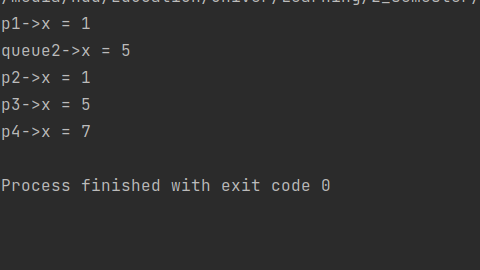
\includegraphics[width=0.8\textwidth]{output.png}
\caption{Результат}
\label{fig:output}
\end{figure}

\end{document}
